\section{Motivação}
Minha ideia original era aprender a utilizar o \LaTeX.
No entanto, é difícil a formatar um texto sem um texto pronto.
Por conta disso, vou reescrever meu pequeno manual sobre VIM e fazer uma extensão com o que aprendi até então.
O uso de um editor específico com certeza simplifica muito as coisas, seja para edição de textos, seja para programação.
Porém, não é sempre que temos máquinas potentes o suficiente para isso.

O pacote de ferramentas que vem com o \LaTeX\ é gigantesco em variedade e em peso.
O pacote de ferramentas que acompanham qualquer outro software de edição de texto o são.
São alguns gigabytes de arquivos, muitas fontes, e diferentes compiladores.
Assustador, mas vamos com calma.
Este pequeno projeto é uma forma de eu me ambientar com o vimtex, e se ajudar alguém, é um ponto extra.

\subsection{Minha Motivação}
Quando comecei a faculdade havia a matéria de introdução à computação.
Nessa matéria sugeriu-se que se instalasse um Linux para fazer os exercícios e entender melhor sobre computação e afins.
De fato funcionou.
Comecei a aprender, e procurar, e aos poucos fui criando uma trilha de aprendizado.
Nessa trilha me encontrei com o terminal, ou prompt de comando, ou shell.
No Linux, é a forma mais eficiente de se executar uma tarefa.
Mesmo que muitas vezes não seja exatamente fácil, é possível salvar em um arquivo de script uma sequência de ações para que seja difícil uma única vez.
Isso me encantou.

Não bastasse isso, eu curso engenharia, e existem contas para se fazer,
procedimentos de cálculo, aproximações e avaliações que podem ser facilitadas com computadores.
Existem diferentes tipos de programas, e todos possuem essa mesma natureza estranha, todos existem dentro de computadores.

\begin{figure}[!h]
\centering

\includegraphics[scale=0.05]{motivacao/laptop-desk-notebook-computer.jpg}
%\label{motivacao_001}
\caption{Computadores são ferramentas.}
\end{figure}

E para finalizar, todas as distribuições Linux conseguem rodar ao menos a linha de comando e um editor de textos.
E o VIM é um editor e tanto.

\subsection{Motivação Para Você}
Se você não dispõe de uma máquina potente, e precisa começar com programação, talvez seja um caminho muito mais difícil o que te espera.
Mas é no caminho mais difícil que temos a evolução mais acentuada.
Aprendi a programar em 2 linguagens de programação, das 3 que conheço, no celular.

Me bastou ter um aplicativo de emulação de terminal.
Tendo no terminal um editor e um compilador, aprendi C, uma das linguagens mais velhas que se tem por aí.
Além disso, fazer exercícios de programação mantém a mente afiada, e exige criatividade.
Com o básico bem estabelecido se chega realmente muito longe.

\begin{figure}[!h]
\centering
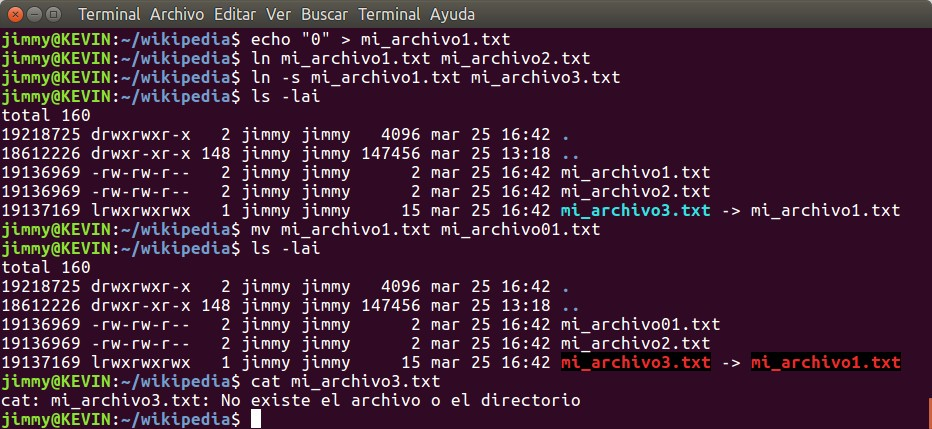
\includegraphics[scale=0.4]{motivacao/Linha_De_Comando.jpg}
%\label{motivacao_002}
\caption{Praticamente todas as máquinas possuem uma interface de linha de comando.}
\end{figure}

Se você possui um computador fraco, pode ser que instalar uma distribuição Linux alivie o peso.
Perde-se muitos aplicativos nativos do Windows, e muitas vezes suas tarefas dependem especificamente do Microsoft Office, ou do AutoCad, ou da suíte Adobe.
Mas também existe a possibilidade de se utilizar programas alternativos.
Existe também uma vantagem didática:
Não existe muita coisa no que prestar atenção para distrair se você está sempre utilizando o mínimo do mínimo.
E mesmo evoluindo na ferramenta, aprende-se compondo conhecimentos anteriores.
Dessa forma, quem aprende a mexer no vim acaba procurando pelos componentes de qualquer editor, para futura instalação e configuração.

Falando de ir além do básico, configurações em servidores são geralmente realizados sem interface gráfica.
Se trata de utilizar um computador distante, especializado em alguma tarefa.
E como eu disse antes, pode ser que pareça difícil, mas basta ser difícil uma única vez.

Uma única recomandação que me parece razoável, é a seguinte: Se você pretende escrever muito no computador, então vale a pena
aprender a digitar da forma correta.
Isso evita lesões por esforço repetitivo, aumenta a velocidade de digitação,
e, com isso, aproxima a velocidade de escrever com a velocidade de pensar.
Digitar enquanto se pensa torna o escrever uma expressão do pensar.

\subsection{Componentes}
O VIM possui pedaços.
E por ele começar tão simples que é uma ótima ferramenta para se evoluir.
Começamos com quase nada, e adicionamos camadas.
Essa construção modular também é o que nos dá a alta capacidade de personalizar.

Outros programas de edição possuem os componentes que podem ser adicionados ao nosso editor favorito.
Outros componentes simplesmente não fazem sentido juntos dessa forma.
Pela versatilidade, e capacidade de se ter numa única ferramenta diversas configurações, decidi me dedicar a aprender.

\subsubsection{Editor de Texto}
O editor de texto é a parte núcleo, que quase todo servidor Linux possui.
Tem-se as funcionalidades básicas: Leitura; Escrita; Busca; Substituição.
E é aí que começa a ficar divertido.
Existe o que se chama de syntax highlighting, a capacidade de exibir o texto
com cores diferentes baseado na sintaxe, no sentido lógico usado.
Essa última característica só está presente caso você instale a versão completa do vim.
Geralmente, a versão padrão do vim que já vem instalada nas distribuições linux é o vim-tiny.

\begin{figure}[!h]
\centering
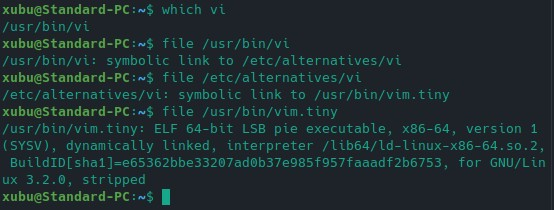
\includegraphics[scale=0.9]{motivacao/VimTiny.jpg}
%\label{motivacao_003}
\caption{O VIM tiny é uma versão de vim simplificada, sem alguns recursos.}
\end{figure}

Além disso, existem formas de se escrever, formas de se pensar, formas de se
mover o cursor pelo texto, que só fazem sentido dentro do vim.
Acontece que essa forma de se pensar é benéfica de tal forma que
editores de código especializados permitem integrar essa forma de se mover.

Temos também a gravação de macros, que são sequências de ações que podem ser
tomadas e repetidas dentro de um texto.
Temos abreviações, que te impedem de escrever a mesma palavra errado e errado novamente,
bastando configurar.
Também pode-se adicionar pequenos trechos de texto que são recorrentes no que se desenvolve.

Pode-se editar arquivos remotamente, pode-se utilizar abas,
e divisões de janela para visualizar mais de um arquivo ao mesmo tempo.
E pode-se invocar um terminal para continuar executando comandos do lado de fora,
enquanto anota-se do lado de dentro.
É muita versatilidade.

\begin{figure}[!ht]
\centering
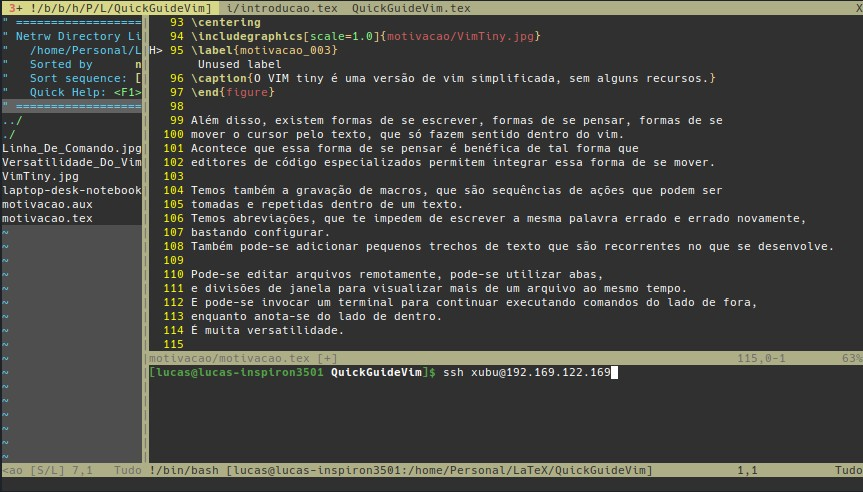
\includegraphics[scale=0.7]{motivacao/Versatilidade_Do_Vim.jpg}
%\label{motivacao_004}
\caption{O VIM completo possui todo tipo de funcionalidade.}
\end{figure}

\subsubsection{Configurações}
Arquivos de configuração fazem loucuras.
Existem templates de configuração, pré configurações
que transformam e aproximam o vim de editores especializados para usos específicos.
Existem configurações que facilitam o uso, e outras que são impossíveis de se desacostumar.
Nos arquivos de configuração, tornam-se persistentes as alterações que também podem ser feitas com o editor aberto.

As configurações permitem alterar atalhos, e existe uma infinidade deles.
Permitem salvar macros, abreviações, mudar esquemas de cores, aparência e ergonomia do uso.
Basicamente, os arquivos de configuração fazem com que o editor fique com a sua cara.
No extremo, chega-se a um ponto em que alguém que também seja conhecido do vim não consiga usar o seu vim.
Nos arquivos de configuração também é onde se deixam plugins ativos.

\begin{figure}[!ht]
\centering
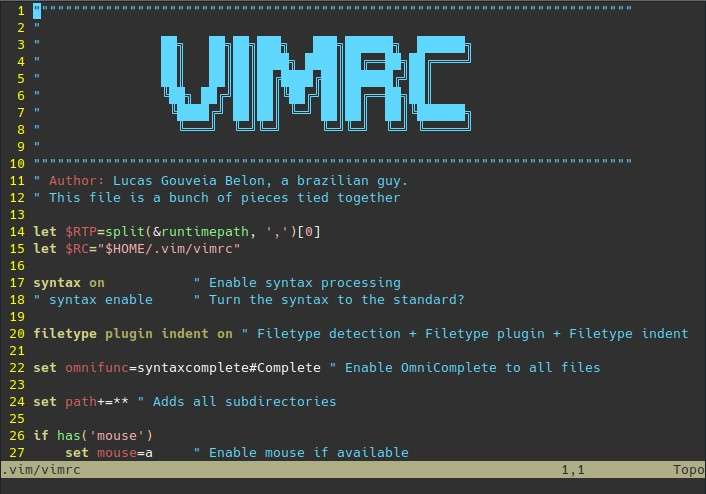
\includegraphics[scale=0.7]{motivacao/Arquivo_De_Configuracao.jpg}
%\label{motivacao_005}
\caption{Arquivo de Configurações do autor.}
\end{figure}

\subsubsection{Plugins}
Para diversos usos, o vim é uma ferramenta tosca.
Não que seja impossível realizar qualquer tarefa com o básico do básico.
Mas se trata de uma ferramenta que começou com funcionalidades limitadas.
E programadores externos ao desenvolvimento da ferramenta possuem formas de
adicionar maneiras mais fáceis de se fazer uma tarefa.
Pensaram novas utilidades nunca antes pensadas, e extensões que se conectam com outros programas.

Talvez seja nos plugins que o vim deixa de ser uma ferramenta ruim para ser sincero.
Vê-se muitos vídeos, tantos vídeos, e blogs, e sites, sobre plugins que fazem isso e aquilo,
que faz parecer que a única função do vim é agregar todos os plugins num único ponto de encontro.

Mas não é bem assim. Existem muitas ferramentas já integradas, e hoje em dia não é tão ruim assim.
Vamos avançar a maior parte do livro sem eles.
Fazer dessa forma talvez mostre quais são os plugins que são essenciais pra você,
ao invés de instalar algo que faz o que já tem embutido, mas de um jeito mais bonitinho.

\begin{figure}[!ht]
\centering
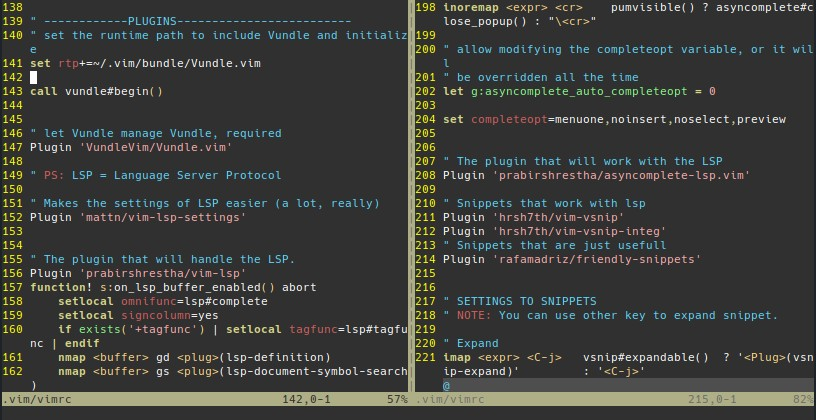
\includegraphics[scale=0.73]{motivacao/Plugin_Exemplo.jpg}
%\label{motivacao_006}
\caption{Plugins do Autor.}
\end{figure}

\subsection{Configurando Máquinas Remotas}
Servidores de dados, de e-mail, servidores web e o mundo na nuvem.
Todos são parte da mesma família de tecnologias.
Aprender uma ferramenta irá te ajudar a entender a próxima, e conseguir aprender mais rápido é motivador.

Essas máquinas remotas podem ser tão simples quanto um computador de 10 anos atrás,
como podem ser super computadores, e ainda assim, não são para propósito geral, são máquinas especializadas.
Não adianta querer jogar nessas máquinas, assim como não adianta querer fazer manobras de skate com uma tábua.
É parecido, mas se trata de outra coisa.

Quando você aprende vim, o suficiente para navegar e fazer todo tipo de coisa doida,
acaba tendo mais domínio e liberdade para fuçar com servidores, ou mesmo com máquinas virtuais.
Veja bem. As próximas imagens serão todas prints de uma máquina virtual linux sem interface gráfica.
Acessarei via ssh, e testaremos juntos os comandos que vou ensinando aos poucos.
Em outras palavras, não vou estar mexendo na minha máquina propriamente dita.

Vamos evitar as configurações o máximo possível, exceto as já comentadas, para sermos capazes de usar
apenas o que já está instalado por padrão.
Mais tarde iremos configurar o NOSSO vim.

Se você chegou até aqui e aturou minha enrolação, então não tem motivo para não ir até o final.
Tentarei ser o mais prático possível.
Planejo fazer de tal forma que você possa abandonar o livro pela metade e se virar muito bem.
Mas muitas funcionalidades interessantes demoraram para serem colhidas e entendidas por esse cérebro
de geleia que está escrevendo. Então, vamos lá.

\newpage
